\section{Microeconomics Midterm 2012 / 13}

{
\subsection*{Schmidt}

\subsubsection*{Exercise 1}

\begin{enumerate}[label=(\alph*)]
{\item 
To violate WA, both bundles must be affordable under both price-wealth-situations:

\begin{align*}
    \left|\begin{array}{c}
    540 \leqslant 360+24 x \\
    30(12+x) \leqslant 600
    \end{array}\right| \\
    \Leftrightarrow \quad\left|\begin{array}{c}
    7.5 \leq x \\
    x \leq 8
    \end{array}\right|
\end{align*}

WA is violated when $x \in[7.5,8]$
}
{\item 
Bundle 2 must be affordable in period 1: $x \leq 8$.
Thus, the consumer prefers bundle 1 to 2 when $x \in[0,7.5)$.
}
{\item 
\color{red} I think he means good 2. \color{black}

As price decreased, we must have a decrease in consumption to satisfy $\frac{\partial x_\ell}{\partial p_\ell}>0$.

Thus: $x<10$

In order to not violate WA, we are left with $x \in[0,7.5) \cup (8,10)$.
}
\end{enumerate}
}

\subsubsection*{Exercise 2}

\begin{enumerate}[label=(\alph*)]
{\item 
Let $f(\cdot)$ be a monotonic transformation and apply Roy's identity to $f(v(p, w))$ :

\begin{align*}
    \tilde{x}_\ell(p, w)
    =-\frac{\frac{\partial f(v(p, w))}{\partial p_\ell}}{\frac{\partial f(v(p, w))}{\partial w}}
    =-\frac{\frac{\partial f(v(p, w))}{\partial v(p, w)} \cdot \frac{\partial v(p, w)}{\partial p_\ell}}{\frac{\left.\partial f\left(p_p, w\right)\right)}{\partial v(p, w)} \frac{\partial v(p)}{\partial w}}
    =-\frac{\frac{\partial v(p, w)}{\partial p_\ell}}{\frac{\partial v(p)}{\partial w}}
    =x_\ell(p, w)
\end{align*}

Even by implementing $f(\cdot)$ we find the same $x_\ell(p, w)$.
}
{\item 
(1) Invert $v(p, w)$ to find $e(p, u)$ :
\begin{align*}
e(p, u)=u\left(\frac{p_1}{\alpha}\right)^\alpha\left(\frac{p_2}{1-\alpha}\right)^{1-\alpha}
\end{align*}
(2) Apply Shepherd's Lemma:
\begin{align*}
\begin{aligned}
h_1(p, u) & =\frac{\partial e\left(p_1 u\right)}{\partial p_1}=u \alpha^{-\alpha}\left(\frac{p_2}{1-\alpha}\right)^{1-\alpha} \alpha p_1^{\alpha-1} \\
& =u\left(\frac{\alpha}{1-\alpha}\right)^{1-\alpha}\left(\frac{p_2}{p_1}\right)^{1-\alpha}
\end{aligned}
\end{align*}
}
{\item 
\begin{align*}
    \text { case 1: } & \alpha=\alpha\left(\frac{p_1}{p_2}\right) \\
    & u_1\left(\lambda p, u\right) = u\left[\frac{\alpha\left(\frac{\lambda p_1}{\lambda p_2}\right)}{1-\alpha\left(\frac{\lambda p_1}{\lambda p_1}\right)} \frac{\lambda p_2}{\lambda p_1}\right]^{1-\alpha\left(\frac{\lambda p_1}{\lambda p_2}\right)} 
    = u \left( \frac{\alpha\left(\frac{p_1}{p_2}\right)}{1-\alpha\left(\frac{p_1}{p_2}\right)} \frac{p_2}{p_1}\right)^{1-\alpha\left(\frac{p_1}{p_2}\right)}=h_1\left(p_1 u\right) \\
    \text { case 2: } & \alpha=\alpha\left(p_1\right) \\
    & u_1\left(\lambda p, u\right) = u\left[\frac{\alpha\left(\lambda p_1\right)}{1-\alpha\left(\lambda p_1\right)} \frac{\lambda p_2}{\lambda p_1}\right]^{1-\alpha\left(\lambda p_1\right)} 
    = u\left[\frac{\alpha\left(\lambda p_1\right)}{1-\alpha\left(\lambda p_1\right)} \frac{ p_2}{ p_1}\right]^{1-\alpha\left(\lambda p_1\right)} \neq h_1\left(p_1 u\right)
\end{align*}
}
\end{enumerate}

\subsubsection*{Exercise 3}

As the returns to scale are constant, we must apply cost-minimization.

\begin{align*}
    \min_x wx \text { s.t. } f(x)=1
\end{align*}

We differentiate with respect to $x_\ell$ to find FOC:

\begin{align*}
    w_\ell-\lambda \frac{\partial f(x)}{\partial x_\ell} &= 0 \\
    w_\ell x_\ell^*-\lambda \frac{\partial f(x)}{\partial x_\ell} x_\ell^* &= 0 \quad \text{use Euler's formula} \\
    w x^*-\lambda \sum \frac{\partial f(x)}{\partial x_\ell} x_\ell^* &= 0 \\
    w x^*-\lambda \cdot 1 &= 0 \\
    w x^*=c(w) &= \lambda
\end{align*}

By constant returns to scale $\min _x wx \text { s.t. } f(x)=y$ will give

\begin{align*}
    w \tilde{x}-\lambda \sum \frac{\partial f(x)}{\partial x_e} \tilde{x}_e &= 0 \\
    w \tilde{x}-\lambda y &= 0 \\
    w \tilde{x}=c(w, y)=\lambda y &= c(w) \cdot y
\end{align*}

\newpage
{
\subsection*{Gottardi}

\subsubsection*{Exercise 1}

\begin{enumerate}[label=(\alph*)]
{\item 
\underline{Consumer A:}

\begin{align*}
    \max _{x^A} x_1^A+2\left(x_2^A\right)^{1 / 2} \text { s.t. } p x_1^A+x_2^A=p 5
    \Longleftrightarrow \max _{x_2^A} 5-\frac{x_2^A}{P}+2\left(x_2^A\right)^{1 / 2}
\end{align*}

First Order Condition:

\begin{align*}
    -\frac{1}{p}+\left(x_2^A\right)^{-1 / 2}=0 \\
    \Leftrightarrow \quad x_2^A=p^2 \rightarrow x_1^A=5-p
\end{align*}

\underline{Consumer B:} 

\begin{align*}
    x_1^B &= \left\{\begin{array}{lll}
    \infty & \text { if } & p<2 \\
    \mathbb{R}^{+} & \text {if } & p=2 \\
    0 & \text { if } & p>2
    \end{array}\right. \\
    x_2^B &= \left\{\begin{array}{lll}
    \infty & \text { if } & p>2 \\
    \mathbb{R}^{+} & \text {if } & p=2 \\
    0 & \text { if } & p<2
    \end{array}\right.
\end{align*}

\underline{Market Clearing:}   

\begin{align*}
    w_1 &= 5=x_1^A+x_1^B=p^2+x_1^B \\
    w_2 &= 6=x_2^A+x_2^B=5-p+x_2^B
\end{align*}

$p=2$ must hold. Otherwise excess demand would not be zero, and markets can't clear.

\underline{Edgeworth Box:}

\begin{figure}[htp!]
    \centering
    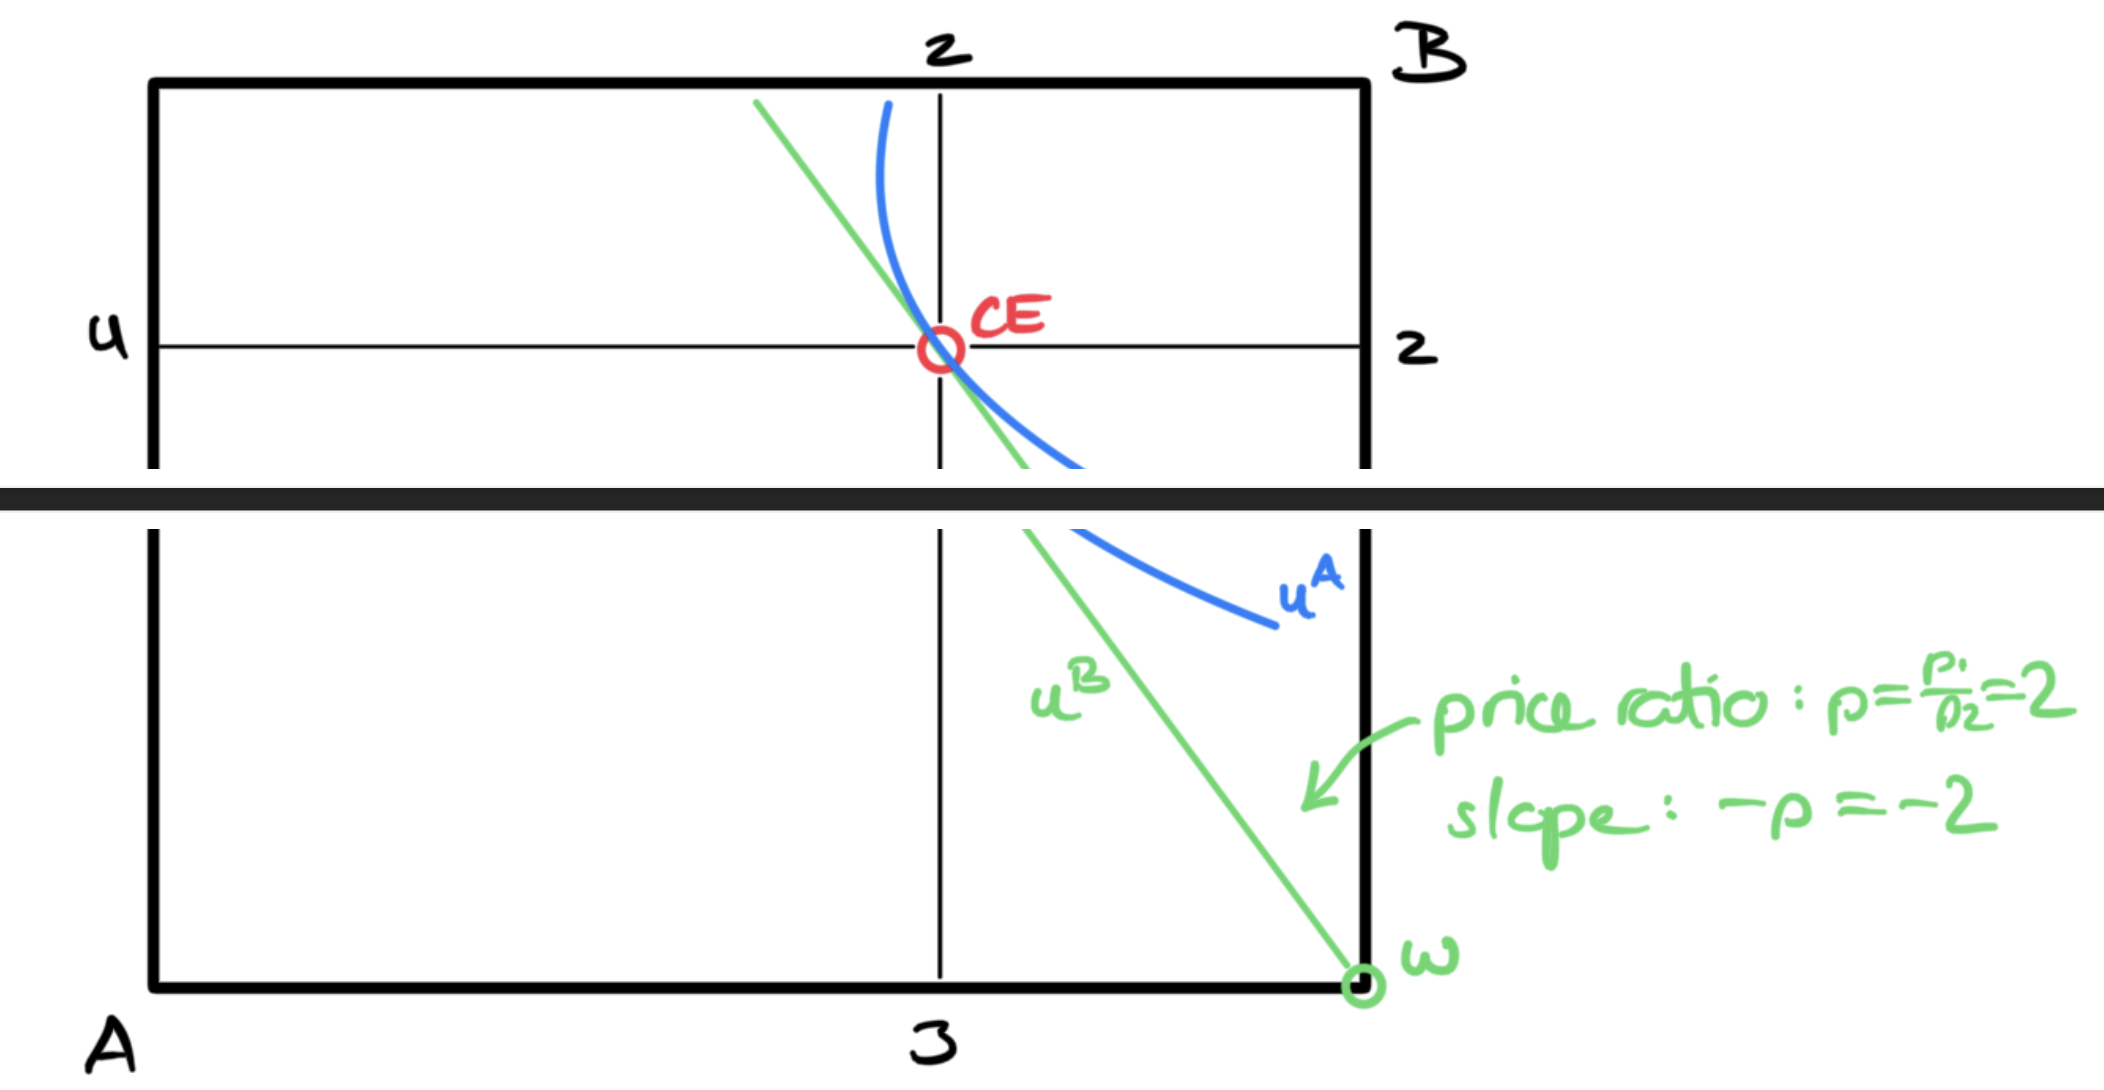
\includegraphics[width=0.75\linewidth]{images/2012_13_edgeworth_box.png}
    \caption{The vertical bar is not part of the figure. The figure was drawn on an iPad and the export created the line. Ignore it.}
\end{figure}
}
{\item 
Agent A cannot influence $x_2^B$. Thus, her FOC does not change: her behaviour is the same. The behavior of agent $B$ does not change as well. Thus, the CE remains the same.
But this CE does not need to be PE anymore, reason being that $X_2^B$ is on externality for A. Incomplete markets lead to inefficient CE allocations.
}
{\item 
\underline{type C:}
Under autarky there's no trade as consumers are identical. Free trade can only lead to a utility increase (or it stays the same) by voluntarity of trade.

\underline{type C:}
If the greater total endowment of good 2 in the economy increases $p$. then A profits as a seller of good 1 .
If price remains at $p=2$, there is no impact.

\underline{type B:}
If $p>2$, $B$ will not sell anything of good 2, and try to buy more of it (which she cannot).
she can't). Then $\left(u^B\right)^{j\text{FT}}=6=\left(u^B\right)^{\text{aut}}$. it $p=2$, also $\left(u^B\right)^{j\text{FT}}=6=\left(u^B\right)^{\text{aut}}$.
}

\subsubsection*{Exercise 2}

Convexity is not needed, but LNS is. Convexity is only needed for the SWT. If LNS is violated, we can immediately construct a counterexample with $L=H=2$:

Although CE exists, we could move south-west to increase B's utility without hurting A.

\begin{figure}[htp!]
    \centering
    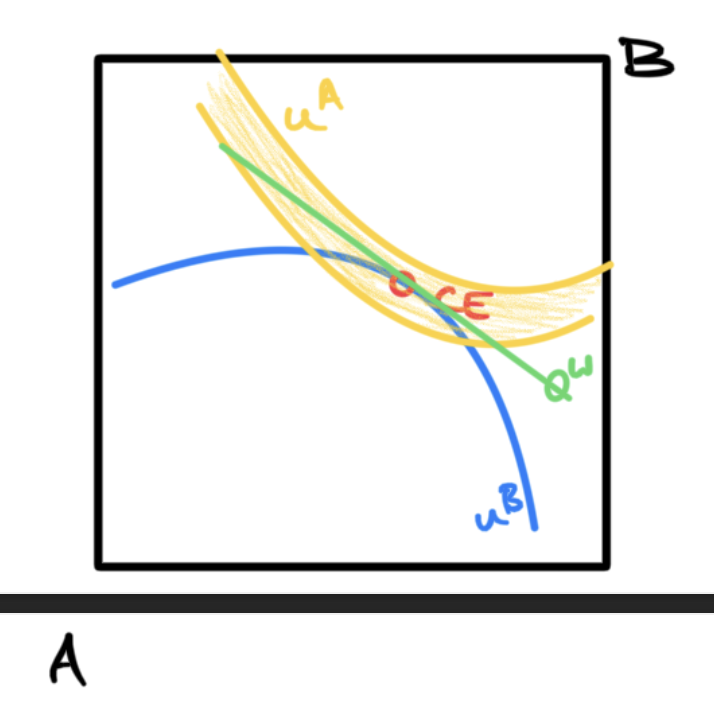
\includegraphics[width=0.75\linewidth]{images/2012_13_counterexample.png}
    \caption{The vertical bar is not part of the figure. The figure was drawn on an iPad and the export created the line. Ignore it.}
\end{figure}

\subsubsection*{Exercise 3}
\begin{enumerate}[label=(\alph*)]
{\item 
\begin{align*}
    w^1=(3,2) \quad w^2=(2,6)
\end{align*}

PE: equalize MRS across consumers.

\begin{align*}
    M R S^1=\frac{\pi(1) \frac{1}{x^{1}(1)}}{\pi(2) \frac{1}{x^1(2)}} 
    &\stackrel{!}{=} M R S^2=\frac{\pi(1) \frac{1}{x^2(1)}}{\pi(2) \frac{1}{x^2(2)}} \\
    \frac{x^{1}(2)}{x^{1}(1)} & =\frac{x^2(2)}{x^2(1)}
\end{align*}

Apply market clearing conditions:

\begin{align*}
    x^2(2) &= 8-x^{1}(2) \\
    x^2(1) &= 5-x^{1}(1)
\end{align*}

Thus: 

\begin{align*}
    \frac{x^{1}(2)}{x^{1}(1)} & =\frac{8-x^{1}(2)}{5-x^{1}(1)} \\
    \frac{8}{x^{1}(2)}-1 & =\frac{5}{x^{1}(1)}-1 \\
    x^{1}(2) & =\frac{8}{5} x^{1}(1)
\end{align*}

\begin{figure}[htp!]
    \centering
    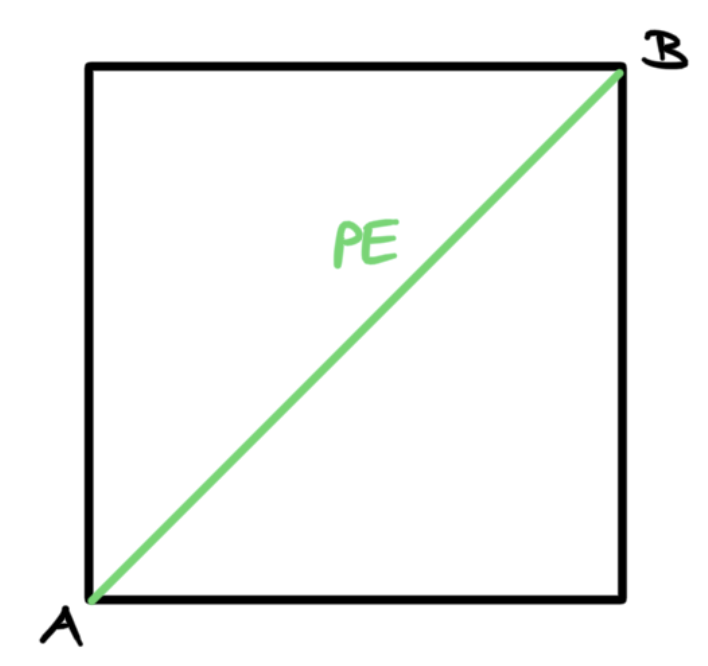
\includegraphics[width=0.5\linewidth]{images/2012_13_PE.png}
\end{figure}
}
{\item 
\underline{consumer h:}

\begin{align*}
    & \max _{x^h} \pi(1) \ln \left(x^h(1)\right)+\pi(2) \ln \left(x^h(2)\right) \\
    & \text { s.t. } \quad p(1)\left(x^h(1)-w^h(1)\right)+p(2)\left(x^h(2)-w^h(2)\right)=0
\end{align*}

The FOCs are

\begin{align*}
& \frac{\pi(1)}{x^h(1)}-\lambda p(1)=0 \\
& \frac{\pi(2)}{x^h(2)}-\lambda p(2)=0 \\
\Longrightarrow\quad &\frac{p(1)}{p(2)}=\frac{\pi(1)}{\pi(2)} \frac{x^h(2)}{x^h(1)} \tag{I}
\end{align*}

Equation (I) describes the relationship of prices and state probabilities. With identical beliefs, we have $\frac{x^{1}(2)}{x^{1}(1)}=\frac{x^2(2)}{x^2(1)}$, ie. PE and thus

\begin{align*}
    \frac{p(1)}{p(2)}=\frac{\pi(1)}{\pi(2)} \frac{8}{5}
\end{align*}

Therefore, in our case we find that $\frac{p(1)}{p(2)}>\frac{\pi(1)}{\pi(2)}$ because total endowment in state 1 is higher than in state 2. If there was greater total endowment in state 1, the inequality sign would switch to $<$. 
}
\end{enumerate}


\end{enumerate}
}
